\documentclass[10pt,letterpaper]{article}

\usepackage{../style/cvpr}
\usepackage{times}
\usepackage{epsfig}
\usepackage{graphicx}
\usepackage{amsmath}
\usepackage{amssymb}
\usepackage{kotex}
\usepackage{multicol}

\usepackage{ifpdf}
\ifpdf
\usepackage{dhucs-cmap}
\pdfmapfile{=myttf-pdftex.map}
\fi
% Include other packages here, before hyperref.

% If you comment hyperref and then uncomment it, you should delete
% egpaper.aux before re-running latex.  (Or just hit 'q' on the first latex
% run, let it finish, and you should be clear).
\usepackage[breaklinks=true,bookmarks=false]{hyperref}

\renewcommand\thesection{\Alph{section}}
\renewcommand\thesubsection{\thesection.\arabic{subsection}}
\renewcommand\thesubsubsection{\thesubsection.\arabic{subsubsection}}

\cvprfinalcopy % *** Uncomment this line for the final submission

\def\httilde{\mbox{\tt\raisebox{-.5ex}{\symbol{126}}}}

\ifcvprfinal\pagestyle{empty}\fi
\begin{document}

%%%%%%%%% TITLE
\title{Automatic Sketch Colorization Using Generative Adversarial Network}

\author{김태범
\qquad
오현석
\qquad
이동재\\
\\
서울대학교 물리천문학부\\
창의적 통합설계 1 중간 보고서 \\
{\tt\small \{k.taebum, \}@snu.ac.kr}
}

\maketitle
%%%%%%%%% ABSTRACT
\begin{abstract}
\end{abstract}


\tableofcontents

\pagebreak
%%%%%%%%% BODY TEXT

\begin{multicols}{2}
\section{Introduction}

딥러닝 기술의 혁신 이후 4차 산업 혁명이라는 말이 생길 정도로 사회에는 큰 변화가 나타났다. 
오로지 사람의 영역으로 여겨졌던 많은 분야에서 점차 사람의 역할을 컴퓨터가 대체하는 현상이 벌어지고 있다. 또한 지금 이 순간에도 컴퓨터의 활용 영역은 조금씩 넓어져 가고 있다. 
본 프로젝트에서 목표로 하고 있는 자동 채색 기술도 그 중 하나이다. 
2000년대 중반 웹툰이라는 플랫폼이 등장하면서 죽어가던 만화 시장에 새로운 활기가 불어넣어졌다. 
이후 웹툰 시장은 급성장하여 일 수백 만 명의 접속자를 기록하며 새로운 문화 플랫폼으로서의 역할을 하게 되었다. 
웹툰의 제작 과정은 크게 스토리 구성, 스케치 및 채색의 과정으로 나눌 수 있다.
최근에는 단순 작화보다는 스토리와 시나리오가 웹툰의 인기 요소로서 더 중요한 역할을 차지하며, 작가들 또한 이러한 트렌드에 맞추어 가고 있다.
이러한 상황 속에서 기계학습을 통한 자동 채색 프로그램이 개발된다면 웹툰 산업에서 놀라운 생산성 증대를 기대해 볼 수 있다. 
또한 웹툰뿐만 아니라 2D 채색이 필요한 게임, 애니메이션 산업 등에서도 널리 활용될 것으로 기대되고 있다.

본 프로젝트에서는 2014년에 딥러닝의 새로운 지평을 열었던 Generative Adversarial Network (GAN) \cite{Goodfellow2014} 를 활용하여 자동 스케치 채색 프로그램을 개발하는 것을 주 목적으로 한다. 
기존에는 GAN을 활용하여 흑백 사진을 채색하거나, 사진을 만화 스타일로 만드는 선행 연구들이 진행되어 왔다.
하지만 이를 실생활에 활용하기 위해서는 흑백 사진이 아닌 단순 스케치를 채색하는 기술이 필요하며, 흑백 사진의 경우 명도와 채도 등의 원래 색의 정보를 어느 정도 가지고 있으므로 스케치 채색에 비해 학습이 잘 이루어지는 편이다. 
즉 기존의 GAN을 이용한 채색 연구에 비해 그 난이도가 높고, 예상되는 활용도 또한 높은 프로젝트이다. 
현재 GAN을 기반으로 하는 \stylepaint~등의 자동 스케치 채색 기술이 알려져 있으며 \cite{Zhang2017}, 3개월간의 본 프로젝트에서는 \stylepaint 를 기반으로 하여 \autopaint~모델 \cite{Liu2018AutoPainter}보다 더 좋은 채색 정확도를 가지는 새로운 모델을 구성하는 것이 궁극적인 목표이다.

본 보고서에서는 현재 알려져 있는 채색 기술에 대해 소개한 후, 포스터 세션으로 이루어진 중간 발표까지의 진행 상황과 앞으로의 계획에 대해 서술하였다. 프로젝트 진행 상황에 대하여 세부적으로는 학습 네트워크의 구성, 데이터셋의 선별과 처리 과정, 그리고 실제 채색 시도 결과에 대하여 서술하였다.

\section{Background Study}


Generative Adversarial Network (GAN) \cite{Goodfellow2014}은 generator가 진짜같은 가짜를 만들고, discriminator가 이 가짜를 진짜와 구분하도록 경쟁적으로 학습시키는 딥러닝의 한 분야이다. 본 프로젝트는 GAN과 관련하여 여러 선행하는 연구들을 참고하며 이루어졌다.
이 장에선, 그 중 주요한 선행 연구들을 소개한다.
먼저 image translation 문제들 전반에 큰 영향을 끼친 \pixpix~연구가 있다 \cite{phillip2017}. 딥러닝 네트워크는 원하는 결과물에 따라 적절한 loss 함수를 선택하는 것이 효율 및 결과에 있어서 중요하다. 기존의 이미지 처리 관련 네트워크들에서는 각 목적에 맞는 특정 loss 함수를 골라 학습을 진행하였는데, 이 논문에서 제시한 네트워크는 주어진 이미지 데이터 쌍에 대하여 input-output image mapping을 학습하는 image-to-image translation 문제들에 대해 일반적인 해답을 제시하였다. 특히 U-Net 구조라는 generator를 제시함으로써, 추후에 나오는 image translation 문제들의 기본이 되는 generator 모델을 제시하였다.
추가적으로, Conditional GAN \cite{Mirza2014CGAN}의 아이디어를 기반으로, 새로운 discriminator인 PatchGAN도 제시하였다.

다음으로 이번 프로젝트의 목표인 sketch colorization에 관한 연구들을 소개한다.
\autopaint 는 \pixpix 를 베이스로 한 모델인데, 광범위한 image translation problem들 중에서 스케치 채색으로 분야를 좁힌 모델이다.
이 모델은 스케치에 어느정도 원하는 색을 입힐 수 있는 방법을 제시하였다 (그림 \ref{fig:autopainter}).
하지만 사용자가 직접 색을 스케치의 각 부분마다 지정해야한다는 점이 단점으로 지적된다.
 
그 외에도 여러 채색 모델들이 존재하는데, 그중에서도 \stylepaint~모델이 성능 및 기능 면에서 가장 뛰어나다 (State-of-the-Art) \cite{Zhang2017}. 이 논문에서는 색칠된 특정 이미지를 style hint로서 스케치와 같이 입력해 주는 것으로 직접 힌트를 제시할 필요 없이 원하는 방식의 색을 입힐 수 있는 네트워크를 제시하였다. 이 네트워크는 \pixpix 의 Redisual U-Net과 ACGAN의 discriminator를 사용하고 \cite{Odena2017}, U-Net의 단점을 보완하기 위한 two Guide Decoders의 구조를 제시하였다. 이 논문은 여러 효과적인 구조 및 학습 방식을 소개하였지만, 모델 구현의 세부적인 사항, 하이퍼파라미터 등을 제공하지 않았고, 또한 여러 자잘한 오류들이 있어 논문에서 제시한 수준의 결과물들을 똑같이 얻어내기 힘든 상황이다.

\begin{figure}[t]
	\centering
	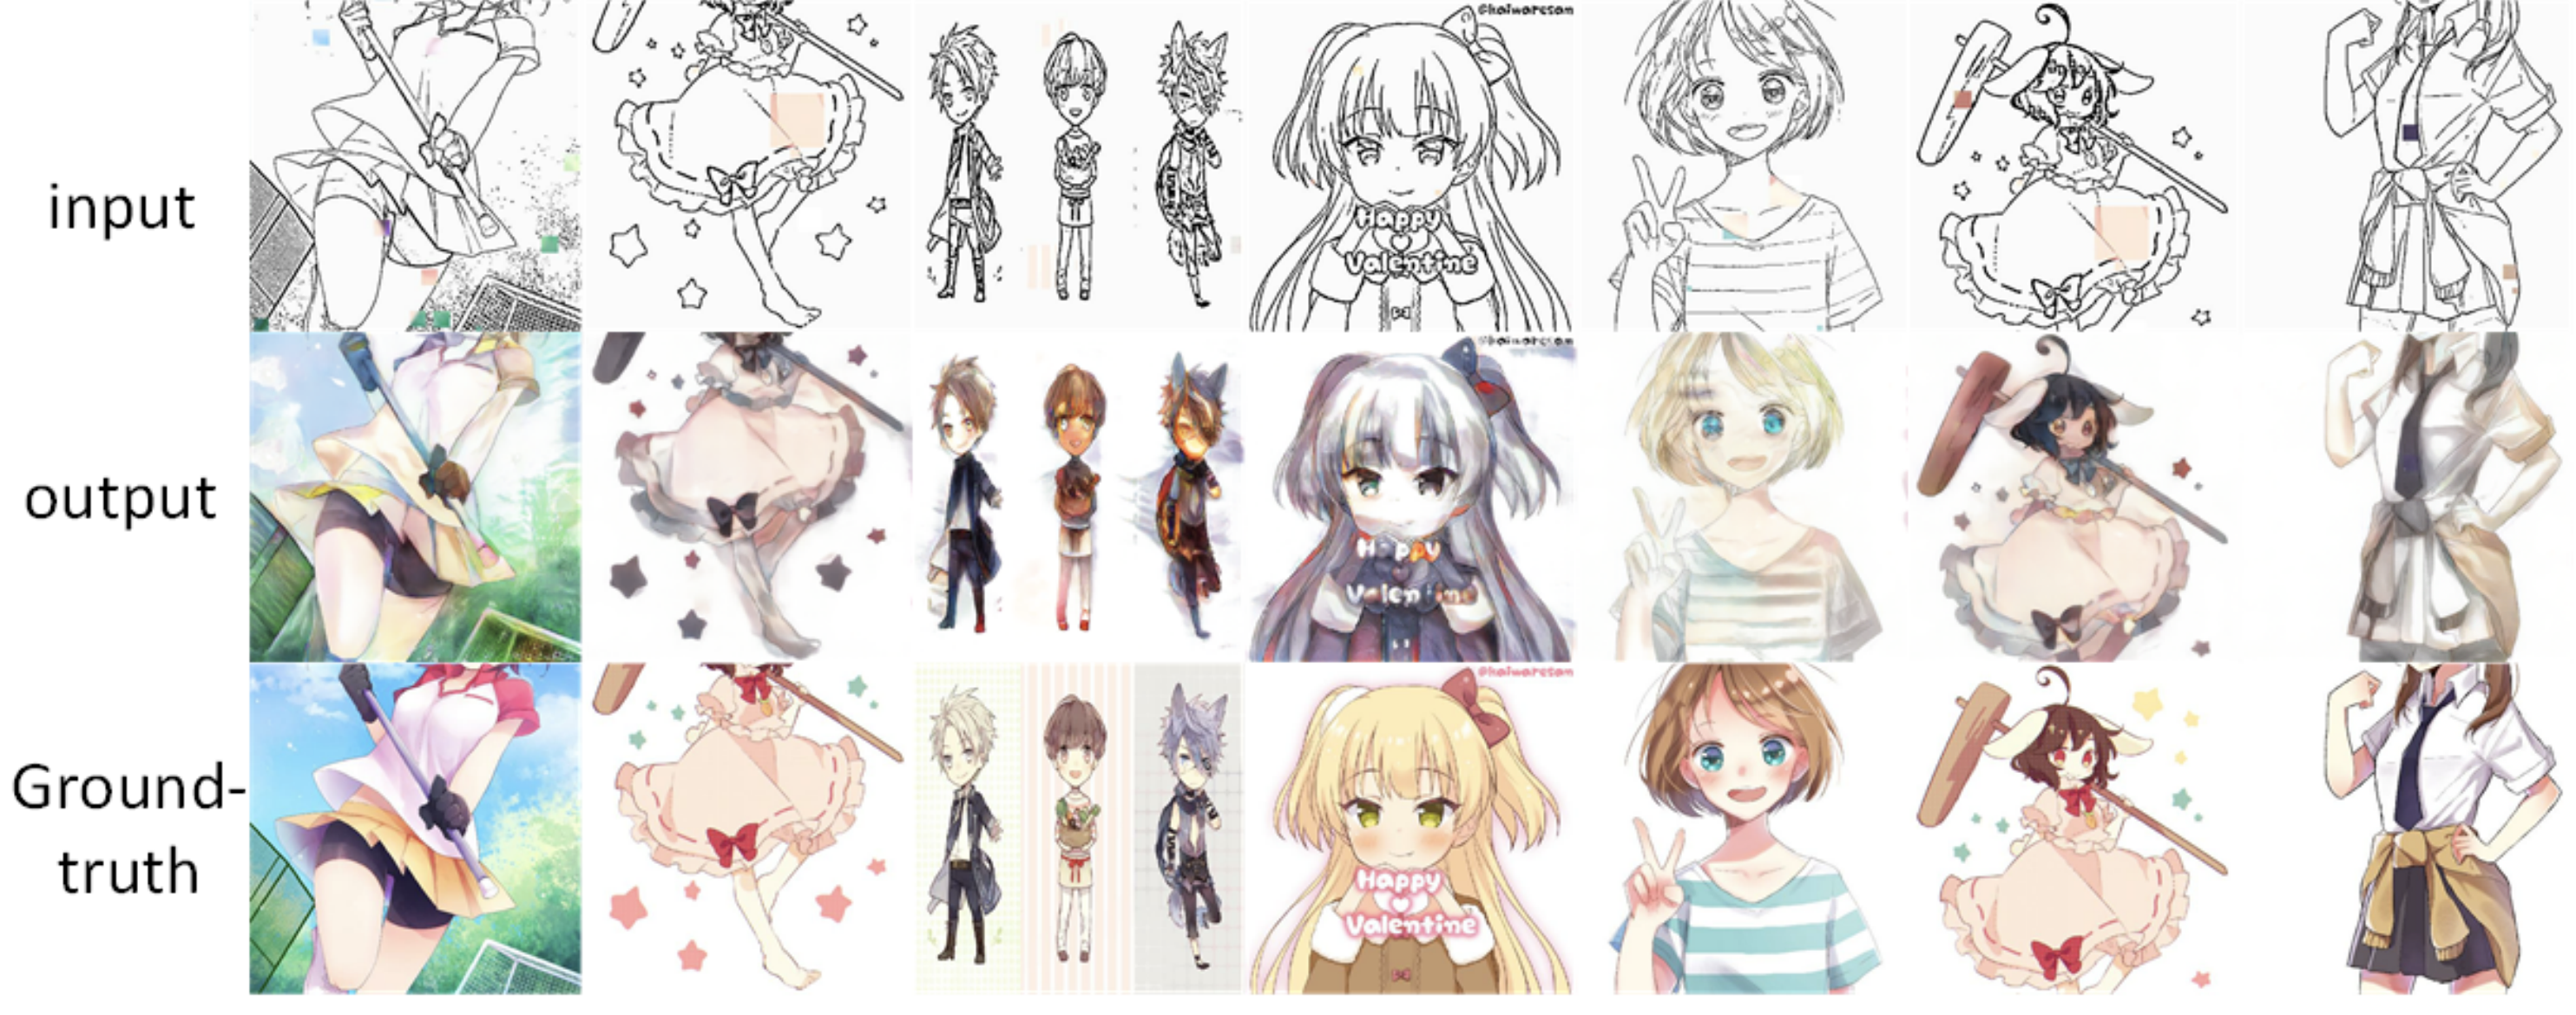
\includegraphics[width=0.9\textwidth]{autopainter}
	\caption{AutoPainter결과 예시}
	\label{fig:autopainter}
\end{figure}
\section{Goal/Problem \& Requirements}

본 프로젝트에서는 현재까지 알려진 채색 모델 중 가장 좋은 성능을 보이는 Style2Paint 모델을 기반으로 하여 AutoPainter 모델을 능가하는 것을 목표로 한다.
Style2Paint 모델은 높은 정확도의 채색 성능을 보이고 있으나, 기본적인 아이디어만 제시되어 있을 뿐 세부적인 구현 내용은 공개되어 있지 않다.
현실적으로 Sytle2Paint의 결과를 100\% 구현하기에는 어려움이 있으므로 다른 초기의 자동 채색 모델 중 비교적 좋은 성능을 보여주는 AutoPainter 모델을 비교 대상으로 설정하였다.

Style2Paint 모델은 U-Net 구조의 generator, VGGNet 기반 Style Extractor, ACGAN의 auxiliary classification discriminator를 사용한다.
이 때 학습과정에서는 스케치와 채색된 이미지의 데이터 쌍이 필요하다.
학습에 필요한 데이터 셋을 바로 구하기는 어렵기 때문에 채색된 이미지로부터 스케치를 추출해내는 과정이 필요하다.
또한 학습에 필요한 모델의 세부 구조와 하이퍼파라미터 값이 정확하게 알려져 있지 않다.
이러한 부분들은 채색 결과에 큰 영향을 미치므로, 좋은 성능을 내도록 이를 최적화하는 과정이 필요하다.
마지막으로 Style2Paint 모델은 style extraction 과정에서 classification 모델을 사용하기 때문에 원하는 스타일의 색 정보가 정확하게 반영되지 못 하는 점이 한계로 지적된다.

본 프로젝트에서는 이러한 문제들을 해결하기 위하여 다음과 같은 세부 목표들을 설정하였다.
\begin{itemize}[topsep=0pt,itemsep=-1ex,partopsep=1ex,parsep=1ex]
	\item 스케치 - 채색 학습 데이터셋의 생성
	\item Style2Paint 모델의 구현 및 최적화
	\item 효율적인 스타일 추출 모델 반영
\end{itemize}
\section{Approach}

더 좋은 모델을 만들기 위해서는, 우선 기존의 모델들에 대한 이해가 충분히 되어야 한다고 판단을 하였다.
따라서 중간평가 기간까지는, 데이터셋을 수집하고, 전처리를 진행하고, 우선적으로 기존의 우수한 채색 모델을 재생산 하는 것에 초점을 두었다.

\subsection{Collect Dataset}

우선 학습을 위한 데이터셋을 위해, 색이 칠해진 에니메이션 그림 데이터셋을 수집하였다.
이 과정에선, style2paint에서 사용하였다고 하는 Niko Open-dataset \cite{ikuta2016}과 Danbooru 2017 Illustration Dataset \cite{danbooru2017}을 함께 사용하였다.

하지만, 이 두 개의 데이터셋은, 인물 그림만 포함하는 것이 아니고, 불필요한 그림들 (풍경 그림, 사진 등)을 함께 포함하고 있다.
그렇기 때문에 우리는, 수작업으로, 우리가 판단하에 쓸만한 데이터들을 분류하였고, 5000장의 이미지 중에서 약 1000장의 이미지를 얻었다.
쓸만한 데이터를 분류한 기준은 다음과 같다.
\begin{enumerate}[topsep=0pt,itemsep=-1ex,partopsep=1ex,parsep=1ex]
	\item 단일 인물, 최대 두 인물의 그림인가?
	\item 배경이 복잡하지 않은가?
	\item 해상도가 너무 크거나 너무 작지 않은가?
\end{enumerate}
이 때, 배경이 복잡하지 않은 것에 대한 기준은, 우선 배경이 흰색인 것을 가장 좋은 그림으로 기준을 잡았고, 학습에 어느정도 일반화를 위하여 단순한 패턴이 들어간 그림이나, 단색 배경도 포함하였다. 해상도에 대한 기준은, 우리는 512 x 512 크기의 이미지에 문제를 한정하였기 때문에, 이보다 작거나, 혹은 너무 큰 이미지는 배제하였다.

\subsection{Preprocessing}

선별한 1000장의 이미지를 우선 8:2로, \textit{train} 데이터셋과 \textit{validation} 데이터셋을 나누었다.
이는 대부분의 딥러닝 모델 학습에서 따르는 비율을 택하였고, 상호 데이터셋 간의 겹치는 이미지 파일은 존재하지 않게 랜덤으로 분배하였다.

\subsubsection{Edge Detection}

이제 전체 데이터셋에 대하여, 우리가 가진 것은 색칠된 (colorized) 이미지 파일들이기 때문에, 학습을 위한 이미지쌍 (sketch, colorized)를 만들고자 하였다. 그러기 위해 잘 알려진 여러 edge detection 알고리즘을 사용하기로 결정하였다.
우리가 선택한 것은 Saining Xie와 Zhuowen Tu가 제안한 Holistically-Nested Edge Detection (HED) \cite{Saining2015}, OpenCv의 Canny Edge Detection \cite{opencv}, 그리고 Python Imaging Library (PIL)의 Edge Detection 알고리즘이다 \cite{pillow}. 각각의 그림의 결과는 그림 \ref{fig:edge_detection}에서 확인할 수 있다.
\begin{figure}[t]
	\centering
	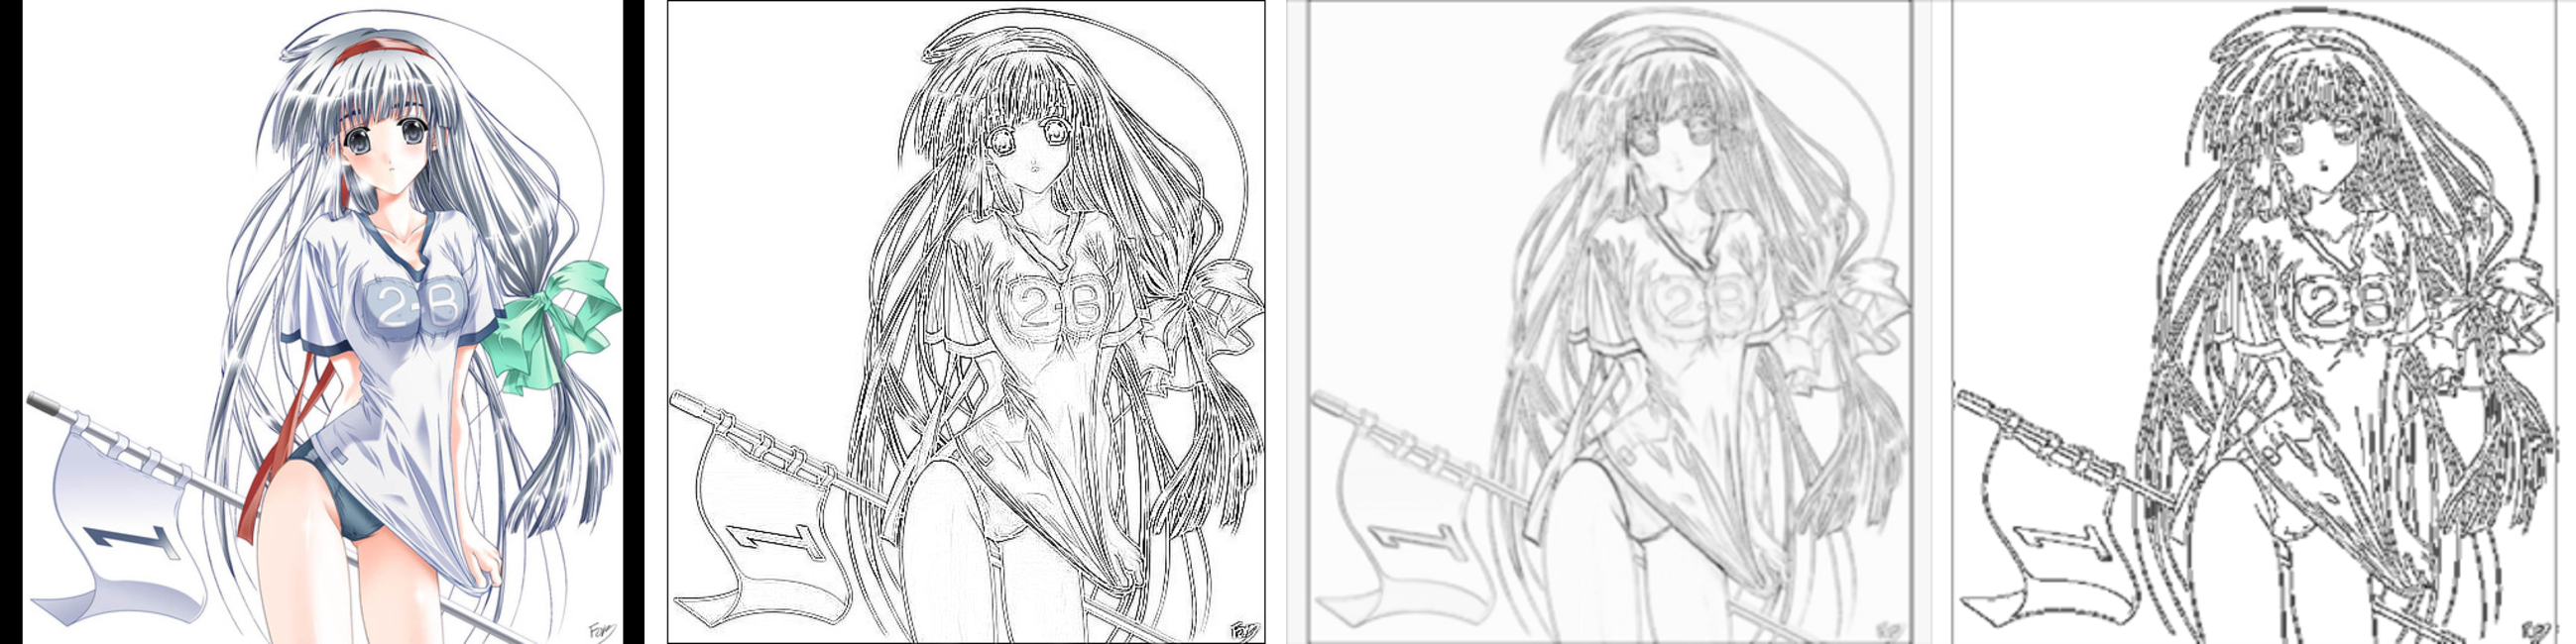
\includegraphics[width=\textwidth]{edge}
	\caption{각각의 edge detection 알고리즘 결과 비교. 가장 왼쪽 그림은 원본 이미지이고, 왼쪽에서 두 번째 그림이 PIL의 결과이다. 왼쪽에서 세 번 그림은 HED, 오른쪽 그림은 Canny Detection 알고리즘의 결과이다}
	\label{fig:edge_detection}
\end{figure}
각각의 결과를 확인한 뒤, 내부 의견 조율로 우리는 PIL의 edge detection 알고리즘을 사용하기로 결정하였다. 

그러나 이 방법만 적용하기에는 스케치라기엔 거친 느낌이 강해서, 이를 완화할 수 있는 추가적인 처리 과정을 강구하였다.
이를 위해 적용한 방법은 두 가지이다.
첫 번째는 Edgar Simo-Serra 외 3명이 제안한 딥러닝 기반의 Sketch Simplification 기술이고 \cite{SimoSerraTOG2018}, 두 번째는 PIL의 자체 이미지 smoothing 필터를 적용하였다.
하지만 Sketch Simplification은 전체적으로 스케치 이미지를 불분명하게 만드는 효과가 있었고, smoothing 필터를 적용한 이미지는, 초기의 거친 느낌을 잡아주었기 때문에, 최종적으로는 PIL edge detection - PIL Smoothing Filter를 sketch 이미지를 만드는 것으로 사용하기로 결정했다 (그림 \ref{fig:edge_smooth}).
\begin{figure}[t]
	\centering
	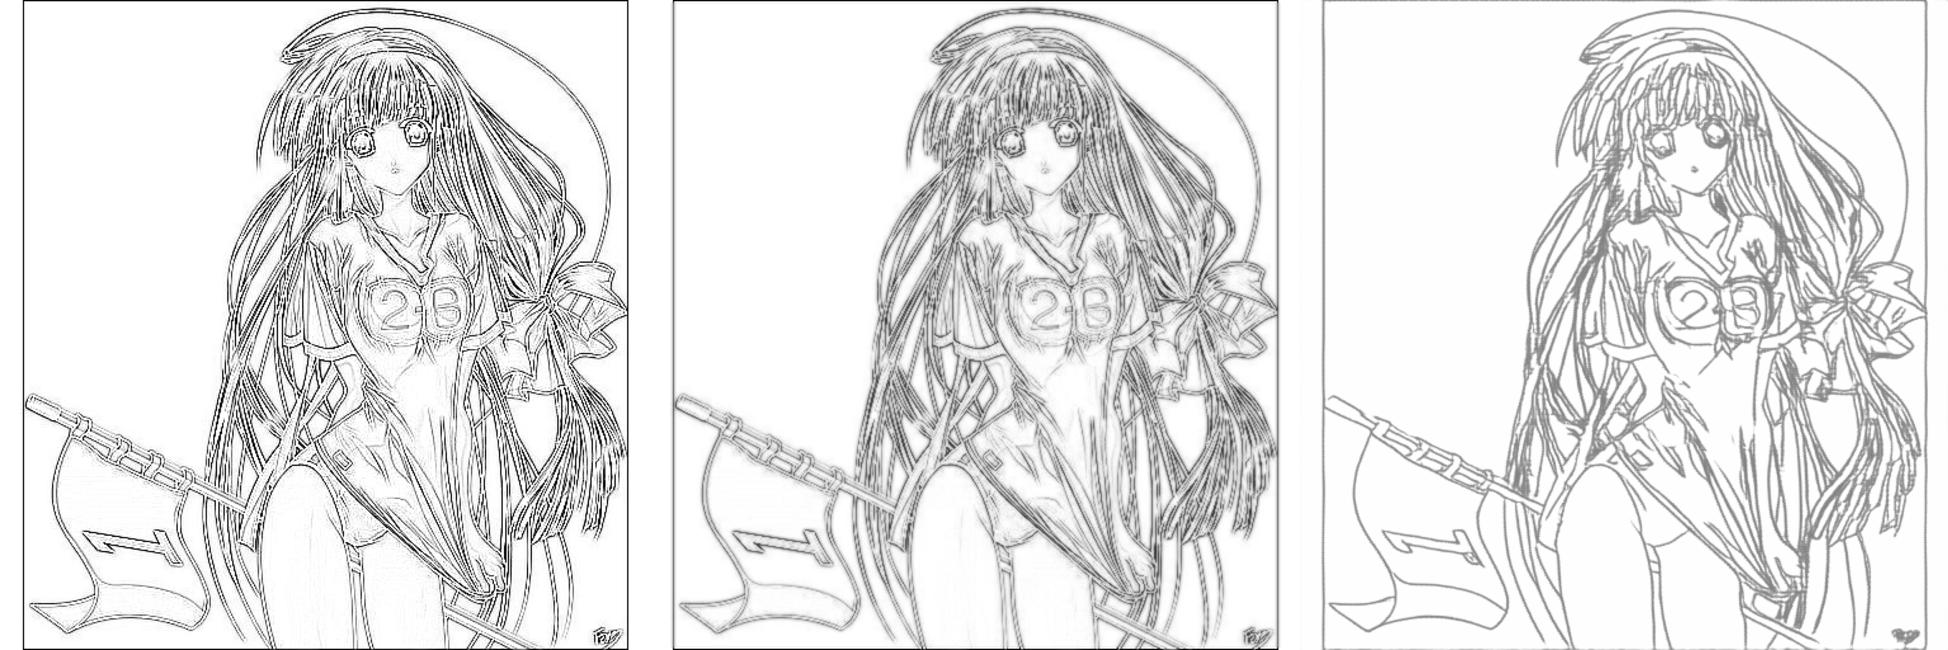
\includegraphics[width=\textwidth]{smooth}
	\caption{PIL edge detection을 통해 얻은 스케치 이미지에 적용한 추가적인 효과. 가장 왼쪽이 edge detection을 통해 뽑아낸 직후이고 (Figure \ref{fig:edge_detection}의 왼쪽에서 두 번째 그림과 동일), 가운데가 이 그림에 Sketch Simplification을 적용한 그림, 가장 오른쪽이 smoothing filter를 적용한 그림이다. 그림에서 확인할 수 있듯이, Sketch Simplification을 적용하면 머리카락 같이 세세하고 많은 스케치를 제대로 잡아내지 못한다.}
	\label{fig:edge_smooth}
\end{figure}

\subsubsection{Image Resizing/Scaling}


\subsection{Model Reproduction}

\subsubsection{Pix2Pix}

\subsubsection{CycleGAN}

\subsubsection{Style2Paint}
\section{Architecture}

\subsection{Generator}

Generator 모델은, 가장 기본적으로는 style2paint에서 제안하는 

\subsection{Discriminator}
\section{Implementation Spec}

\section{Current Achievement}

이전 장에서 기술한 구현 내용으로 실험을 진행하였고, 이에 대한 결과는 그림 \ref{fig:current}에서 확인할 수 있다.
하지만 그림 \ref{fig:current}을 자세히 보면, 첫 번째 이미지 같은 경우, 사람이 전체적으로 초록색과 검은색으로 색칠되었음을 확인할 수 있다.
하지만 목표 스타일 이미지를 보면, 옷은 조금 더 초록색으로, 다리는 살색으로, 얼굴은 살색, 머리는 노란색으로 색칠이 되는 게 현실적이고 자연스러운 스타일 적용이라고 볼 수 있다.
이는 현재 모델의 Style Extractor가 224 x 224 크기의 이미지를 input으로 받고, 현재 구현된 모델은 주어진 이미지의 중심을 기준으로 224 x 224 이미지로 잘라서 넣었기 때문에, 모델 입장에서는 스타일 이미지의 가운데 부분 (그림 \ref{fig:center}) 만 볼 수 있게 된다. 직관적으로도 이는 전체적인 스타일 적용은 힘들 것으로 생각이 되고, 앞으로 개선해야할 문제점이라고 인식하였다.

또한, 그림 \ref{fig:current}의 두 번째, 세 번째 그림을 보면, 스케치의 배경은 단색이지만, 채색된 결과를 보면, 배경에 대해서는 불필요한 노이즈들이 채색되는 것을 확인할 수 있다.
따라서 우리는 이러한 부분도, 노이즈가 없는 깔끔한 배경으로 색칠이 되게 해야할 필요성을 느꼈다.
\begin{figure}[t]
	\centering
	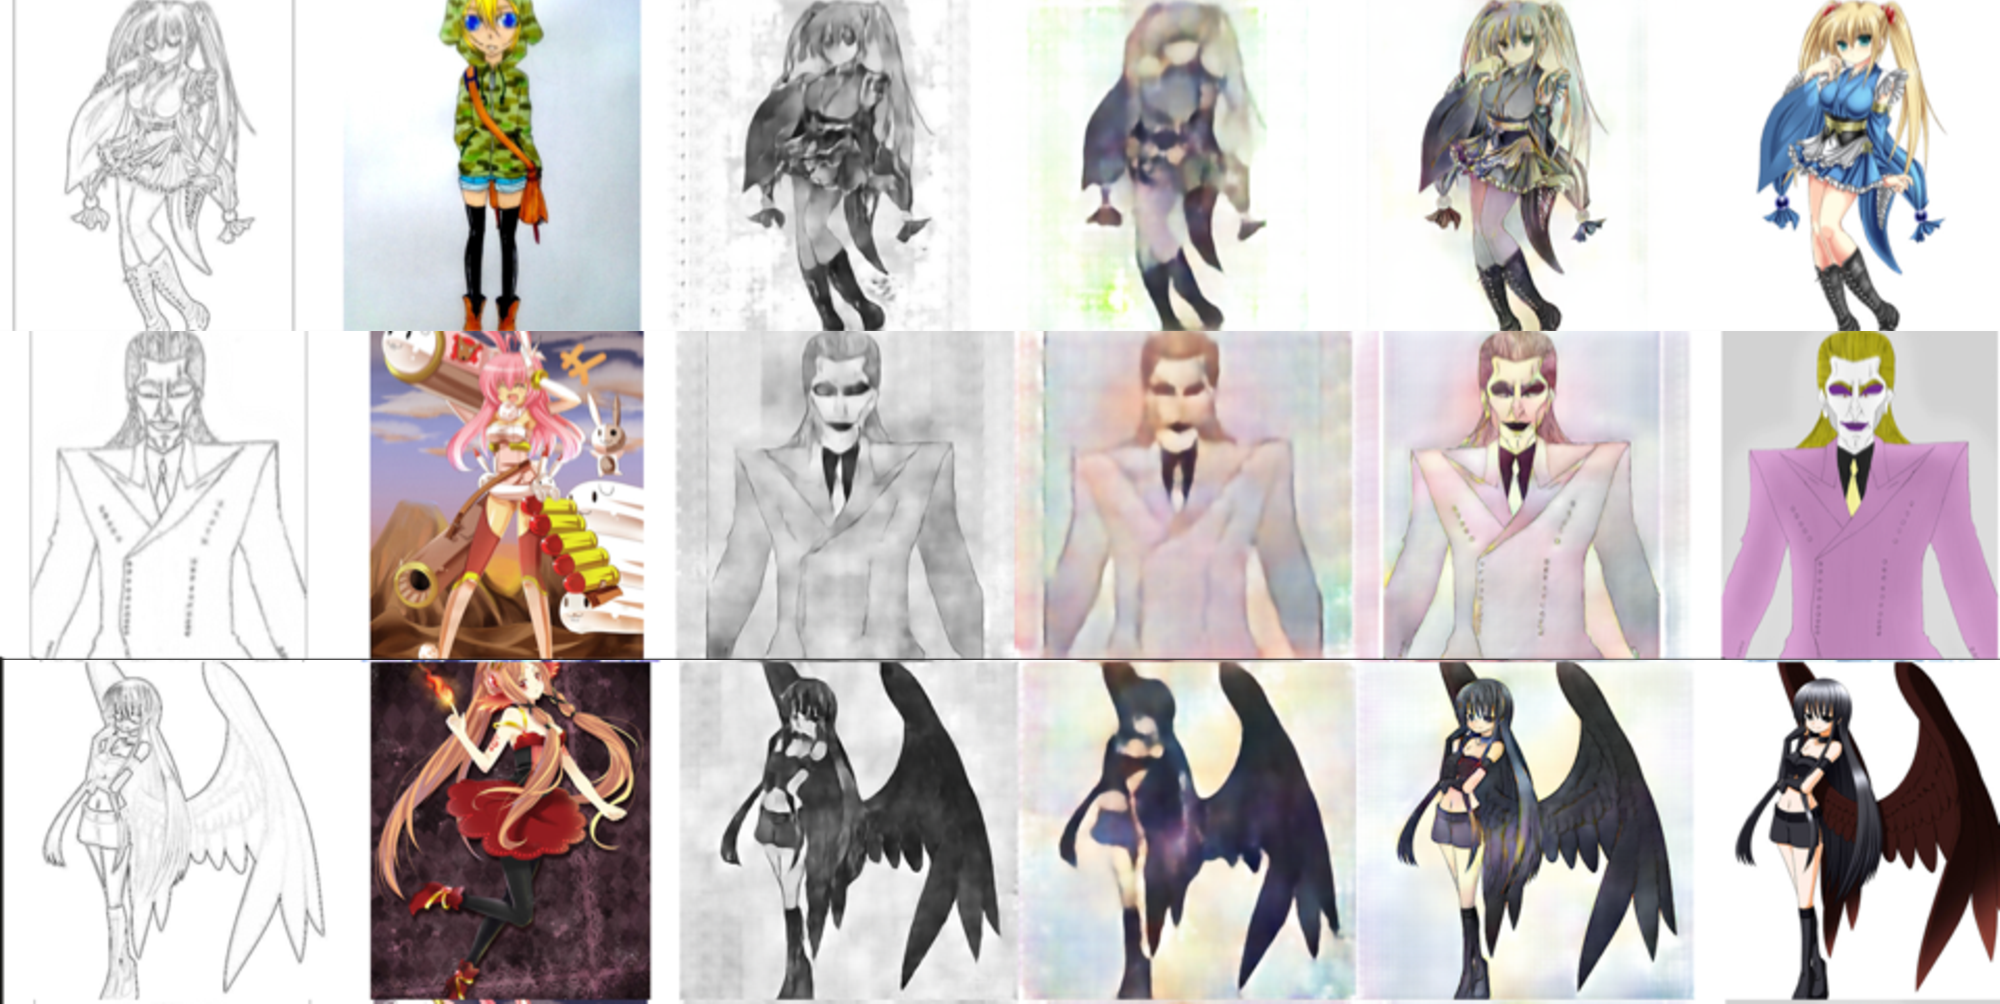
\includegraphics[width=\textwidth]{result}
	\caption{style2paint를 기반으로 한 모델 실험 결과. 가장 왼쪽부터, 주어진 스케치 이미지, 목표 스타일 이미지, Guide Decoder1의 결과, Guide Decoder2의 결과, 채색 결과, 원래 이미지이다.}
	\label{fig:current}
\end{figure}

\begin{figure}[t]
	\centering
	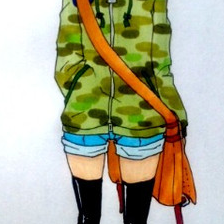
\includegraphics[width=0.2\textwidth]{center}
	\caption{그림 \ref{fig:current}의 첫 번째 스타일 이미지에서, 이미지의 중심을 기준으로 224 x 224 크기로 자른 부분. 현재 Style Extractor는 이 부분만 참고한다.}
	\label{fig:center}
\end{figure}


\section{Future Work}

이 섹션에서는 중간발표 이후의 계획에 대하여 서술한다.
교수님의 의견인 '확실한 스펙의 부재'의 문제를 해결해야할 필요성을 느꼈고, 이에 대해서 다음과 같이 앞으로 진행할 방향을 수정하기로 하였다.

\subsection{Colorize Part by Part}

style2paint를 reproduce하면서 이 논문에서 제안하는 방법을 우리의 문제 상황에 그대로 적용하기에는 다음과 같은 차이점 및 문제가 있다고 판단을 하였다.

첫 번째로는 이미지 해상도에 의한 차이이다. style2paint 논문은 학습시 이미지의 크기를 256 x 256 pixel 이미지로 제한을 하였다.
하지만 우리는 더 좋은 해상도인 512 x 512 pixel 이미지를 목표로 잡았기 때문에, 이에 따른 문제들이 발생한다. 결정적인 문제는, style extraction을 할 때 VGGNet \cite{Simonyan2014}에 들어가는 이미지의 해상도는 224 x 224이다.
현재로써는 주어진 style 이미지에 대해, 이미지의 가운데로부터 224 x 224 크기만큼 잘라서 Style Extractor에 input으로 넣었기 때문에, Style Extractor는 전체적인 이미지 스타일을 보지 못 하고, 일부분만 보게된다. 그렇기 때문에, 채색을 할 때, style 이미지의 얼굴 부분은 얼굴 부분대로, 몸 부분은 몸 부분대로 들어가지 못 하고 부자연스러운 결과를 나타낸다.

이에 대해, 우리는 현재 잘 알려진 Object Detection Network를 사용하여 \cite{Ross2015, Ross2014,Kaiming2017, Joseph2016}, 주어진 그림 속에서 얼굴과, 몸을 각각 2개의 224 x 224 크기의 bounding box로 detection 할 수 있는 추가적인 모델 구현을 할 것이다. 정확하게 얼굴과 몸을 detect 할 수 있게되면, 채색 모델을 학습할 때, 얼굴에 대한 style extract, 몸에 대한 style extract를 각각 적용할 것이고, 이를 통해서 조금 더 현실적인 채색이 가능할 것이라고 생각된다.

\subsection{Model Improvement}

현재까지 실험에서는 discriminator를 pix2pix에서 제시한, PatchGAN을 사용하였다 \cite{phillip2017}.
하지만, style2paint 논문에서는 PatchGAN은 성능이 좋지 않고 Auxiliary Classifier GAN (ACGAN) \cite{Odena2017}이나, Deep Convolutional GAN (DCGAN) \cite{Radford2015}를 사용했다고 언급이 되어있다.
그렇기 때문에, 이와 같은 discriminator 모델을 사용하여 실험을 진행하는 것이 가치가 있을 것이라 판단된다.

또한 Generator에서도 현재 512 x 512 해상도의 이미지에 대해 적용을 하므로, 기존의 모델보다는 조금 더 깊은 모델에 대해 실험을 해보는 것이 가치가 있을 것으로 판단된다. 따라서 더 깊은 모델을 구현할 때 높은 성능을 보장한다고 알려진 Residual Network \cite{He2016ResNet}와 Dense Network \cite{Huang2017DenseNet}의 기술을 적용했을 때의 결과를 확인할 것이다.

마지막으로, loss 함수 및 하이퍼파라미터 조정에 따른 실험 결과도 관찰할 것이다.
현재는 GAN loss를 제외하면 L1 loss를 사용하고 있는데 style transfer에서 사용하는 Content Loss \cite{Gatys2015StyleTransfer}등을 이용하면, 채색 결과에 차이가 있을 것으로 예상된다.
이 과정들을 통해 어느정도 채색의 정확도가 높아진다면, 지속적인 하이퍼파라미터 조정을 통해, 실제 사용할 수 있는 모델을 만들 계획이다.
\section{Division \& Assignment of Work}

\section{Schedule}


\begin{table}[H]
	\caption{프로젝트 타임 테이블}
	\begin{center}
		\begin{tabular}{|L{4cm}|C{0.3cm}|C{0.3cm}|C{0.3cm}|C{0.3cm}|C{0.3cm}|C{0.3cm}|C{0.3cm}|C{0.3cm}|C{0.3cm}|C{0.3cm}|C{0.3cm}|C{0.3cm}|C{0.3cm}|}
			\toprule
			\multirow{2}{*}{\textbf{내용}} 
			&\multicolumn{3}{|c|}{\textbf{9월}}&\multicolumn{4}{|c|}{\textbf{10월}}&\multicolumn{4}{|c|}{\textbf{11월}}&\multicolumn{2}{|c|}{\textbf{12월}}\\
			\cline{2-14}
			&2&3&4
			&1&2&3&4
			&1&2&3&4
			&1&2\\	
			\toprule
			GAN 모델 사전 학습 
			& \cellfill & \cellfill & \cellfill 
			& \cellfill & & &
			& & & &
			& & \\
			\midrule
			데이터셋 수집 및 처리
			& & & \cellfill
			& \cellfill & \cellfill & \cellfill & \cellfill
			& & & &
			& & \\
			\midrule			
			기존 모델 구현
			& & &
			& & \cellfill & \cellfill & \cellfill
			& & & &
			& & \\
			\midrule
			새로운 모델 설계
			& & &
			& & & \cellfill & \cellfill
			& \cellfill & \cellfill & &
			& & \\
			\midrule
			모델 분석 및 성능 향상
			& & &
			& & & &
			& \cellfill & \cellfill &\cellfill &\cellfill 
			& & \\
			\midrule
			성능평가
			& & &
			& & & &
			& & & \cellfill & \cellfill
			& \cellfill & \cellfill \\
			\midrule
			최종 발표
			& & &
			& & & &
			& & & &
			& & \cellfill \\
			\bottomrule
		\end{tabular}
	\end{center}
	\label{tab:multicol}
\end{table}



{\small
\bibliographystyle{ieee}
\bibliography{egbib}
}
\end{multicols}
\end{document}


